
Die praktische Ausarbeitung stellt ein \textit{Proof of Concept} dar, also ein Machbarkeitsnachweis der im theoretischen Teil hergeleiteten L\"osungsans\"atze. Die Schwerpunkte sind die parallele Ausf\"uhrung verschiedener Aktionen, die dynamische Erweiterung durch Module sowie die Ausprogrammierung und Herleitung der Theorien f\"ur das Host-Discovery\index{Host-Discovery}, die Anordnung der Systeme innerhalb eines Hypercubes\index{Hypercube}, die Alert-\"Ubermittlung und Pr\"ufung sowie die Performance im Allgemeinen.

Als Modell f\"ur die Programmierung und die generelle Entwicklung des \"Uberwachungs-Systems wird eine Mischform aus Experimentellem- sowie Evolution\"arem-Protoyping und einer spiralf\"ormigen Entwicklung gew\"ahlt. Dies bedeutet, dass Funktionen mittels der Software ausprobiert, verbessert und analysiert, jedoch auch wieder entfernt oder komplett anders gestaltet werden k\"onnen. Das kann in Zusammenarbeit mit Endanwendern oder auf Grund von Tests und Analysen geschehen. Die Verbesserung der Performance sowie des Funktionsumfanges wird jedoch eher in einem spiralf\"ormigen Prozess ablaufen. Die Grundfunktionen des Systems werden also relativ gering ausfallen und sind unter Umst\"anden auch noch nicht optimal implementiert. In verschiedenen Zyklen werden je nach Bedarf neue Funktionen und Schnittstellen implementiert oder die Performance von solchen verbessert und angepasst.

Durch diese Vorgehensweise\index{Vorgehensweise} wird das System nicht nur anwenderfreundlich, sondern auch die Performance wird nur an den Stellen verbessert, an welchen es \"uberhaupt sinnvoll ist. Der Weg von der hier entwickelten Technologie-Demonstration zu einem fertigen Produkt ist anschliessend nur ein kleiner.

Das Grundsystem\index{Grundsystem} muss schon von der Basis aus sehr performant laufen, es sollte so wenig Rechenleistung und Speicher wie m\"oglich ben\"otigen. Aus diesem Grund, und um nicht auf die Vorteile der Objektorientiertheit zu verzichten, wird als Programmiersprache Vala\cite{vala}\index{Vala} eingesetzt und keine Interpreter-/Skript-Sprache oder C\#/Java welche eine VirtualMachine als Laufzeitumgebung voraussetzen. Vala ist eine an C\#\index{C\#} angelehnte, objektorientierte Programmiersprache\index{Objektorientiert}, deren Compiler den Vala-Code zuerst in reinen C-Code umwandelt und diesen anschliessend kompiliert. Auf anderen Betriebssystemen\index{Betriebssystem} und Architekturen kann entweder der erzeugte C-Code oder auch direkt der Vala-Code kompiliert und anschliessend verwendet werden. Die einzige Voraussetzung ist, nebst der Einhaltung gewisser Paradigmen, dass es Vala, die GLib\cite{glib}\index{GLib} sowie Gee\cite{gee}\index{Gee} und GIO\cite{gio}\index{GIO} f\"ur die entsprechende Plattform und Architektur gibt.


%%%%%%%%%%%%%%%%%%%%%%%%%%%%%%%%%%%%%%%%%%%%%%%%%%%%%%%%%%%%%%%%%%%%%%%%%%%%%%%%%%%%%%%%%%%%%%%%%%%%%%%%%%%%%%%%%%%%%%%%%%%%%%%%%%%%%%%%%
\section{Grundsystem} \label{sec:praxis-basis}
Das Grundsystem\index{Grundsystem}, siehe Abbildung \ref{fig:praxis-aufbau}, stellt die zentrale Plattform des \"Uberwachungs-Systems dar. Die zentrale Einheit bildet dabei das \texttt{MainSystem}\index{MainSystem}, welches nicht nur globale Funktionen zur Verf\"ugung stellt, sondern auch als Schnittstelle\index{Schnittstelle} zwischen den einzelnen Bereichen fungiert. Um diesen System-Kernel\index{System-Kernel} angeordnet befinden sich die Bereiche zur Daten\"ubertragung (Netzwerk-und Bus-Technologien), zur \"Uberwachung von Diensten und Systemen (\"Uberwachungsmodule), zur Datenspeicherung, f\"ur das Melden von Vorkommnissen (Alerting) sowie Schnittstellen f\"ur die Datenanzeige auf Remote-Systemen (Remote-API). Diese verschiedenen Bereiche werden als Module implementiert und nur bei Bedarf geladen. Die Module k\"onnen sowohl in bin\"arer Form als auch als LUA-Skript\index{LUA}\footnote{LUA\cite{lua} ist eine imperative Skriptsprache welche sich einfach erweitern und einfach in C-Programme einbinden l\"asst. Vorteil von LUA-Skripten ist die Plattformunabh\"angigkeit\index{Plattformunabh\"angig}, sowie die M\"oglichkeit, einfachen Code zu schreiben welcher mit dem vorhandenen System \"uber eine definierte Schnittstelle kommunizieren kann.} vorliegen - wobei die LUA-basierenden Module nicht im Rahmen der Thesis implementiert werden.

\begin{figure}[h]
  \centering
  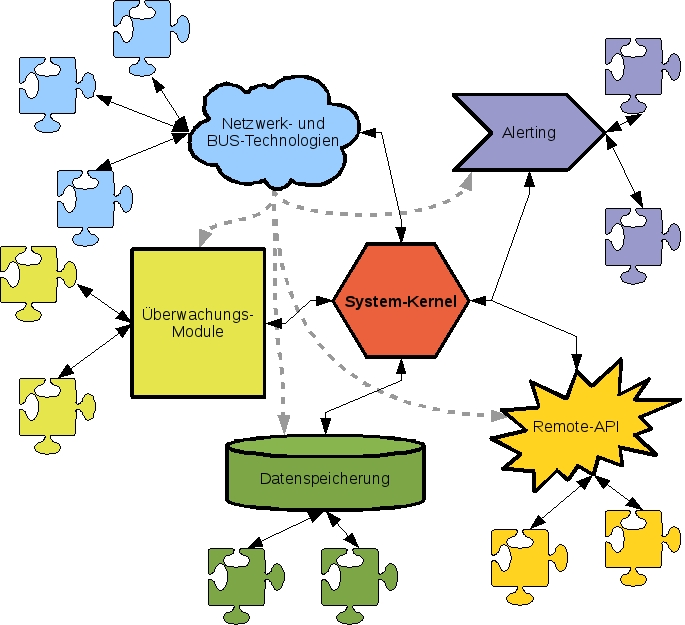
\includegraphics[width=0.8\linewidth]{images/theorie/Aufbau_Grundsystem}
  \caption[Aufbau der \"Uberwachungs-Software]{Das \"Uberwachungs-System bietet rund um den zentralen System-Kernel verschiedene Funktionen f\"ur unterschiedliche Bereiche an. Diese verschiedenen Bereiche stellen jeweils Container f\"ur Module dar, welche sowohl in bin\"arer Form als auch als LUA-Skript vorliegen k\"onnen. Eine Modul-Instanz kann beim System-Kernel eine Instanz eines anderen Moduls anfragen und dieses direkt nutzen. Dieser Prozess ist mit den "`Netzwerk- und BUS-Technologien"'-Modulen schematisch dargestellt.}
  \label{fig:praxis-aufbau}
\end{figure}

\subsection{System-Kernel} \label{sec:praxis-basis-kernel}
Die zentrale Schnittstelle\index{System-Kernel}, der System-Kernel, ist grunds\"atzlich verantwortlich f\"ur die komplette Thread-Verwaltung\index{Thread-Verwaltung} sowie f\"ur die Kommunikation zwischen den Threads und den Modulen.

Nach dem Start des Programms wird eine Instanz des System-Kernels angelegt und die verschiedenen Modul-Container\index{Modul-Container} geladen. Sind alle Modul-Container erfolgreich geladen, wird zuerst der \texttt{MainSystem}-Thread\index{MainSystem}, anschliessend der \texttt{Monitoring}-Thread\index{Monitoring} und zum Schluss der \texttt{MainListener}-Thread\index{MainListener} gestartet. Die verschiedenen Threads werden in den nachfolgenden Kapiteln beschrieben.

Durch einen Z\"ahler, welcher beim Erstellen einer Modul-Container Instanz inkrementiert wird, sowie einem Signal, welches der Conatiner sendet, wenn alles geladen ist, kann gepr\"uft werden, ob alle Container geladen worden sind. Vor der Initialisierung wird also ein Z\"ahler inkrementiert sowie eine Funktion des System-Kernels an das Signal gebunden (Codeblock \ref{alg:praxis-basis-kernel-container-init1}). Konnten alle Module erfolgreich geladen werden, wird vom Container das Signal aufgerufen und dadurch die vorg\"angig daran gebundene Funktion. Diese Funktion dekrementiert den Z\"ahler und f\"uhrt weitere Ladeaktionen aus wenn dieser wieder bei $0$ angelangt ist (Codeblock \ref{alg:praxis-basis-kernel-container-init2}).

Der Thread des \texttt{MainSystem} dient vor allem dazu, eine Asynchrone MessageQueue\index{MessageQueue} ab zu arbeiten. Nachrichten in dieser Queue k\"onnen von unterschiedlichen Stellen eingespiesen werden. Eine Nachricht\index{Nachricht} besteht immer aus einem Kommando und optionalen Daten (siehe Codeblock \ref{alg:praxis-basis-kernel-msg}). Die Nachrichten werden nach dem FIFO-Prinzip (first in first out) abgearbeitet, sie werden also der Reihe nach ausgelesen und das darin enthaltene Kommando ausgef\"uhrt. Sind keine Daten mehr in der \texttt{MessageQueue}, wird der Vorgang f\"ur 100ms pausiert. In einer zuk\"unftigen Version kann angedacht werden, anstelle der Pausierung f\"ur 100ms diesen komplett zu stoppen und beim einspeisen einer Nachricht ein Signal ab zu setzen, welches den Thread wieder aufweckt.

Eine weitere Aufgabe des \texttt{MainSystem}-Threads\index{MainSystem} sind diverse Aufr\"aumarbeiten. Bei einem Host-Discovery\index{Host-Discovery}\index{Discovery} wird beispielsweise eine Objekt-Liste mit verschiedenen Discovery-Prozessen (siehe Kapitel \ref{sec:praxis-basis-discovery}) angelegt. Ist ein Prozess abgeschlossen, muss dieser beendet und wieder freigegeben werden.

\subsubsection{Globale Kernel-Funktionen} \label{sec:praxis-basis-global}
Zur Kommunikation mit den unterschiedlichen Modulen und den verschiedenen Modul-Containern\index{Modul-Container} stehen im System-Kernel\index{System-Kernel} einige \"offentliche Funktionen zur Verf\"ugung:
\begin{description}
\item[exit](): Beendet alle Threads und das Programm\index{Funktionen!exit}

\item[getComm](string name): Erzeugt ein neues Kommunikations-Modul (ICommModule) und gibt dieses zur Verwendung zur\"uck.\index{Funktionen!getComm}\index{Modul!Kommunikation}

\item[getData](string name): Erzeugt ein neues Datenbank-Modul (IDataModule) und gibt dieses zur Verwendung zur\"uck.\index{Funktionen!getData}\index{Modul!Daten}

\item[getAlert](string name): Erzeugt ein neues Alert-Modul (IAlertModule) und gibt dieses zur Verwendung zur\"uck.\index{Funktionen!getAlert}\index{Modul!Alerting}

\item[getRemote](string name): Erzeugt ein neues Remote-API-Modul (IRemoteModule) und gibt dieses zur Verwendung zur\"uck.\index{Funktionen!getRemote}\index{Modul!Remote-API}

\item[getMonitor](string name): Erzeugt ein neues Monitoring-Modul (IMonitorModule) und gibt dieses zur Verwendung zur\"uck.\index{Funktionen!getMonitor}\index{Modul!Monitoring}\index{Monitoring!Modul}

\item[logMonitoring](string plugin, string host, string$\left[ \right]$ result): Nimmt eine Meldung von einem \"Uberwachungsmodul entgegen und speichert diese in allen konfigurierten Datenbanken ab.\index{Funktionen!logMonitoring}\index{Monitoring!Nachricht speichern}

\item[sendAlert](string plugin, string host, int timeout, string subject, string short\_message, string message, string$\left[ \right]$ attachment=null): Nimmt eine Fehlermeldung entgegen und sendet einen Alert wenn dies erforderlich ist. Basierend auf dem Plugin und dem Host kann gepr\"uft werden, ob ein Alert schon versendet worden ist oder nicht. Die Parameter werden 1:1 an das entsprechende Alert-Modul \"ubergeben. Je nach Art der Nachricht werden die einzelnen Daten dabei gek\"urzt oder erst gar nicht versendet.\index{Funktionen!sendAlert}\index{Monitoring!Alert speichern}

\item[getDiscoverServiceList](): Gibt eine Liste mit allen Diensten zur\"uck, auf welche ein System gepr\"uft werden soll, wenn dieses beim Auto-Discovery gefunden worden ist. Die Liste besteht aus \texttt{Helper.NetService}-Datens\"atzen.\index{Funktionen!getDiscoverServiceList} Die \texttt{Helper.NetService}-Datenstruktur ist im Anhang \ref{alg:praxis-basis-netservice} zu sehen.

\item[setDiscoveredHosts](Helper.NetService$\left[ \right]$ list): Systeme, welche durch ein AutoDiscovery gefunden und untersucht worden sind, k\"onnen \"uber diese Funktion dem System mitgeteilt werden. Die Systeme m\"ussen als \texttt{Helper.NetService} vorliegen.\index{Funktionen!setDiscoveredHosts}

\item[getDataFile](string file\_name): Gibt ein \texttt{File}-Objekt f\"ur eine Datei oder ein Verzeichnis innerhalb des "`data"'-Verzeichnisses zur\"uck.\index{Funktionen!getDataFile}

\item[getPath](string$\left[ \right]$ name): Gibt ein Unterverzeichnis als String zur\"uck. Die Unterverzeichnisse m\"ussen als String-Array \"ubergeben werden.\index{Funktionen!getPath}

\item[getFile](string$\left[ \right]$ path, string name): Gibt eine Datei als String zur\"uck. Die Unterverzeichnisse m\"ussen als String-Array \"ubergeben werden.\index{Funktionen!getFile}
\end{description}

\subsubsection{Modul-Container / PluginRegistrar} \label{sec:praxis-basis-kernel-container}
Ein Modul-Container\index{Modul-Container} ist prinzipiell eine einfache typisierte Liste, welche ein bin\"ares Modul laden und Instanzen von diesem zur\"uckgeben kann. Diese typisierte Liste wird implementiert durch den \texttt{PluginRegistrar}. Beim Instanzieren muss das Verzeichnis angegeben werden, welches die Module beinhaltet, die geladen werden sollen. Existiert das angegebene Verzeichnis, werden alle Unterverzeichnisse der Reihe nach durchlaufen und in diesen nach der Datei \texttt{libplugin.so}\index{libplugin.so} gesucht. Existiert eine solche Datei, wird sie in den Speicher geladen und versucht \"uber die Funktion \texttt{register\_plugin(Module module, PluginRegistrar registrar)}\index{Funktionen!register\_plugin} das Plugin zu initialisieren. Diese Einstiegsfunktion muss das Plugin durch den Typen, den Pfad sowie einen Identifier im entsprechenden \texttt{PluginRegistrar}\index{PluginRegistrar} speichern. Wird keine solche Einstiegsfunktion gefunden, kann das plugin nicht geladen werden.

Bei der Initialisierung eines \texttt{PluginRegistrar} muss immer auch ein Interface angegeben werden, welches f\"ur die geladenen Module verwendet wird. Zus\"atzlich muss auch noch ein Pointer auf das \texttt{MainSystem} \"ubergeben werden, so dass die Module und auch der Container Anfragen an den System-Kernel stellen k\"onnen (siehe Codeblock \ref{alg:praxis-basis-kernel-container-init1}).

Damit der \texttt{PluginRegistrar}\index{PluginRegistrar} andere Komponenten dar\"uber informieren kann, dass nun alle Module geladen sind, wird nach dem Laden ein Signal abgesetzt. Auf dieses Signal k\"onnen sich andere Komponenten Funktionen registrieren, welche anschliessend aufgerufen werden (siehe Codeblock \ref{alg:praxis-basis-kernel-container-init1} und \ref{alg:praxis-basis-kernel-container-init2}). Durch diese Funktionalit\"at stellt der System-Kernel fest, wann alle Module geladen sind und mit dem Laden von anderen Komponenten und Threads weitergemacht werden kann.

\begin{figure}[h]
 \lstset{language=[ISO]C++}
 \begin{lstlisting}[label=alg:praxis-basis-kernel-container-init1,caption={[Initialisierung eines Modul-Containers]Dieser Modul-Container l\"adt alle Module im Verzeichnis \texttt{pnetwork} und ruft nach dem erfolgreichen Laden die Funktion \texttt{modulesLoaded} (siehe Codeblock \ref{alg:praxis-basis-kernel-container-init2}) aus dem MainSystem auf. Durch den \texttt{load()}-Aufruf wird der Ladevorgang gestartet.}]
// Counter to check if all Container are loaded
registrars_loaded++;

comm = new PluginRegistrar<ICommModule>("pnetwork", this);
comm.complete.connect(modulesLoaded);
comm.load();
 \end{lstlisting}
\end{figure}

\begin{figure}[h]
 \lstset{language=[ISO]C++}
 \begin{lstlisting}[label=alg:praxis-basis-kernel-container-init2,caption={[Pr\"ufung, ob bereits alle Modul-Container geladen sind]Eine Funktion, die an das \texttt{complete}-Signal des \texttt{PluginRegistrar} gebunden wird, muss \"uber den Parameter \texttt{string path} verf\"ugen. Dieser beinhaltet den Pfad der Module. Diese Implementierung zeigt, wie gew\"ahrleistet wird, dass erst nach dem Laden aller Container gewisse Funktionen ausgef\"uhrt werden.}]
private void modulesLoaded(string path) {
  registrars_loaded--;

  // All modules are loaded
  if (registrars_loaded <= 0) {
    ...
  }
}
 \end{lstlisting}
\end{figure}

Jedes Plugin, das geladen wird, registriert sich entweder \"uber die Funktion \texttt{addPlugin(""IMainModule ""plugin)} oder \"uber \texttt{addInstance(""Type t, ""string path, ""string identi""fier)} bei dem Modul-Container. Ein Plugin kann sich dadurch als "`bereits instanziert"' oder als "`noch zu instanzieren"' registrieren. Durch die Festlegung, dass ein \"Uberwachungssystem so wenig Resourcen wie m\"oglich belegen darf, sollten bereits instanzierte Plugins so wenig wie m\"oglich genutzt werden, da diese beim Systemstart komplett in den Speicher geladen werden und dort verbleiben (w\"ahrend dem die anderen geladen und anschliessend wieder freigegeben werden). Zudem sollte ein solches Plugin als Singelton implementiert werden, denn es kann nur einmal im System bestehen.

Plugins, welche \"uber die \texttt{addInstance(...)}-Funktion registriert werden, k\"onnen zu einem beliebigen Zeitpunkt instanziert werden. Daf\"ur notwendig ist lediglich der Typ, welcher der Funktion \"ubergeben wird. Damit dies jedoch funktioniert, muss beim Laden der Datei \texttt{libplugin.so} angegeben werden, dass dieses Modul speicherresistent sein muss, ansonsten wird der Speicher mit den Modul-Informationen beim verlassen der Funktion wieder freigegeben. Codeblock \ref{alg:praxis-basis-kernel-container-load} zeigt einen schematischen Ablauf des Ladeprozesses. Bei Zeile 4 und 7 wird das Plugin \"uber ein Modul geladen und auf Zeile 9 definiert, dass die Informationen speicherresistent gehalten werden m\"ussen. Anschliessend wird bei Zeile 12 gepr\"uft, ob die Einstiegsfunktion \texttt{register\_plugin} existiert. Ist dies nicht der Fall, wird abgebrochen. Auf den Zeilen 16 und 17 wird der Typ der Einstiegsfunktion definiert und diese anschliessend bei Zeile 18 aufgerufen.

\begin{figure}[h]
 \lstset{language=[ISO]C++}
 \begin{lstlisting}[label=alg:praxis-basis-kernel-container-load,caption={[Beispiel zum Laden eines bin\"aren Moduls]Ablauf zum Laden eines bin\"aren Modules. Zuerst wird das Modul geladen, speicherresident gehalten, auf die Einstiegsfunktion gepr\"uft und diese, wenn gefunden, aufgerufen.}]
protected delegate Type RegisterPluginFunction(Module module,
                                    PluginRegistrar registrar);

string plugin_file = Module.build_path(
    Path.build_filename(module_dir.get_path(), plugin_name),
    "plugin");
Module module = Module.open(plugin_file,
                            ModuleFlags.BIND_LAZY);
module.make_resident();

void* function;
if (!module.symbol("register_plugin", out function)) {
  return;
}

RegisterPluginFunction register_plugin =
   (RegisterPluginFunction)function;
register_plugin(module, this);
 \end{lstlisting}
\end{figure}

Basierend auf dem Identifier\index{Plugin-Identifier}, welcher jedes Plugin pro Modul-Container\index{Modul-Container} eindeutig macht, kann der System-Kernel anschliessend eine Instanz eines Moduls anfragen. Ist das Plugin im angefragten ModulContainer vorhanden, wird basierend auf dem Typen ein neues Objekt erstellt, auf das dem \texttt{PluginRegistrar}\index{PluginRegistrar} zugrunde liegende Interface gecastet und zur\"uckgegeben (siehe Codeblock \ref{alg:praxis-basis-kernel-container-get}). Wird ein nicht existierendes Modul angefragt, wird anstelle dessen \texttt{NULL} zur\"uckgegeben. Es muss also immer zuerst gepr\"uft werden, ob die angefragte Instanz \texttt{NULL} ist oder nicht. Ansonsten kann es zu Problemen bei der Programm-Ausf\"uhrung und zu Instabilit\"aten kommen (\texttt{NULL}-Pointer Exceptions, Assertions, etc.).

\begin{figure}[h]
 \lstset{language=[ISO]C++}
 \begin{lstlisting}[label=alg:praxis-basis-kernel-container-get,caption={[Erstellen einer neuen Instanz eines Moduls]Nachdem alle Module geladen worden sind, kann ein Modul \"uber die Funktion \texttt{getPlugin(string name)} angefordert werden. Existiert ein Plugin mit dem Identifier \texttt{name}, wird eine Instanz von diesem zur\"uckgegeben. Vor der R\"uckgabe wird das neu erstellte Objekt auf das dem PluginRegistrar zugrundegelegte Interface gecastet.}]
public class PluginRegistrar<T> : Object {
  public T? getPlugin(string name) {
    if (pluginExists(name))
      return (T)new Object(ModuleType(name));
    return null;
  }
}

// Get an ICMP-Plugin
ICommModule mod = comm.getPlugin("icmp");
 \end{lstlisting}
\end{figure}

\subsubsection{Monitoring-Thread} \label{sec:praxis-basis-kernel-monitor}
Damit weder ein anderes System noch anderen Komponenten der Software vom Monitoring ausgebremst oder unterbrochen werden, wird dieses in einen eigenen Thread ausgelagert. Das Monitoring\index{Monitoring} l\"auft somit parallel zu allen anderen Funktionen, kann jedoch den System-Kernel ungehindert verwenden.

Nach dem Start des Threads durch den System-Kernel\index{System-Kernel} werden alle Monitoring-Systeme und Module geladen, konfiguriert und im Speicher in einer Liste gehalten. In regelm\"assigen Abst\"anden wird dann diese Liste durchlaufen und geschaut, welche Pr\"ufung aktuell ansteht. Ob ein System zum aktuellen Zeitpunkt durch das momentane Modul gepr\"uft werden soll oder muss, wird dabei nicht vom Monitoring-Thread bestimmt, sondern vom Modul selbst. Jedes Modul weiss, wann es zuletzt ausgef\"uhrt worden ist und wann der n\"achste Zeitpunkt f\"ur eine Pr\"ufung ist (siehe Kapitel \ref{sec:praxis-basis-monitor}). Der Monitoring-Thread schaut grunds\"atzlich nur, ob das Modul aktuell eine Pr\"ufung durchf\"uhrt oder nicht sowie ob der Zeitpunkt (Timestamp) des Moduls abgelaufen ist. Basierend auf diesen zwei Tatsachen kann dann gesagt werden, ob eine Pr\"ufung ansteht oder nicht.

Der Monitoring-Thread kann durch den System-Kernel \"uber das Property \texttt{pause} unterbrochen respektive pausiert werden. Dies hat den Sinn, dass wenn zum Beispiel neu zu \"uberwachende Hosts eingef\"ugt werden, diese vom Monitoring-Thread zuerst geladen werden m\"ussen (definiert \"uber das Property \texttt{reload}). Damit es bei solchen Aktionen nicht zu Datenfehlern kommt, wird bei einem Rebuild der \"Uberwachung dieser Thread pausiert und anschliessend wieder neu gestartet, respektive der Mainloop des Threads wird wieder ausgef\"uhrt.

\subsubsection{Kommunikations-Thread} \label{sec:praxis-basis-kernel-listener}
Damit die verschiedenen \"Uberwachungssysteme untereinander kommunizieren k\"onnen, wird der MainListener-Thread\index{MainListener} gestartet, welcher f\"ur diese Kommunikation zust\"andig ist. Nachrichten unter den Systemen werden mit dem verbindungslosen Protokoll UDP versendet, damit ein allenfalls nicht laufendes System nicht die komplette \"Uberwachung ausbremst\footnote{Bei TCP-Verbindungen kann es vorkommen, dass eine Verbindung, welche nicht korrekt oder komplett aufgebaut werden kann, diese erst nach einem definierten Timeout geschlossen wird oder so lange versucht wird diese korrekt auf zu bauen bis eben dieses Timeout abgelaufen ist. W\"ahrend dieser Zeit ist das System ausgebremst, da es ja eine Antwort erwartet.}. Zudem darf ein System nicht ausgebremst werden, wenn ein anderes System ausgelastet ist und das erstellen einer Antwort mehrere Sekunden in Anspruch nimmt. Bei einer TCP Verbindung wird immer eine Antwort ben\"otigt, was bedeutet, dass das anfragende System ausgebremst wird f\"ur die Dauer welche das ausgelastete System f\"ur die Erstellung der Antwort braucht. Bei UDP k\"onnen Antworten nicht direkt sondern m\"ussen ebenfalls als UDP-Paket versendet werden. Somit spielt es bei UDP keine Rolle, wie lange ein System f\"ur die Erstellung einer Antwort braucht.

Der Thread beinhaltet einen UDP-Listener-Socket\index{UDP}, welcher auf alle vorhandenen NICs (Network Interface Card) gebunden ist. Das Problem bei UDP-Sockets ist, dass immer angegeben werden muss, wie viele Bytes empfangen werden sollen. Aus diesem Grund k\"onnen Daten nicht einfach so wie sie vorliegen gesendet werden, sondern m\"ussen gegebenenfalls in mehrere Pakete aufgeteilt und empfangen werden. Eine Gr\"osse, welche sich bei UDP etabliert hat, sind 1024 Bytes\index{UDP-Paketgr\"osse}. Diese Anzahl scheint Tests zufolge auf den meisten Systemen performant zu laufen, w\"ahrend gr\"ossere Pakete bei gewissen Betriebssystemen Schwierigkeiten bereiten\footnote{Ein UDP-Paket von 2048 Bytes brauchte auf einem WindowsXP fast doppelt so lange wie zwei UDP-Pakete mit 1024 Byte.}.

Aus diesem Grund musste ein einfaches und simples Datenformat definiert werden, welches Abbildung \ref{fig:praxis-basis-kernel-listener-format} aufzeigt. Aktuell werden alle Daten als Klartext versendet, was nicht nur viel Datenmenge bedeutet, sondern auch sicherheitskritisch sein kann. Kommende Versionen der Software sollten nicht nur eine komprimierte oder bin\"are Version des Protokolls aufweisen, sondern auch eine Authentifizierung und/oder sogar eine Verschl\"usselung.

\begin{figure}[h]
  \centering
  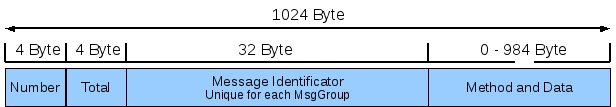
\includegraphics[width=0.8\linewidth]{images/theorie/Aufbau_Kommunikation_Format}
  \caption[Datenformat einer AMoDS-Meldung]{Jeweils 4 Zeichen definieren die aktuelle Nachrichtennummer und die totale Anzahl an Nachrichten. Die folgenden 32 Zeichen werden als Nachrichten-UID interpretiert. Die restlichen 984 Zeichen sind die Daten, welche das Kommando getrennt durch einen Doppelpunkt von den Daten beinhalten.}
  \label{fig:praxis-basis-kernel-listener-format}
\end{figure}

Alle UDP-Pakete, die auf einem definierten Port eingehen, werden empfangen und auf G\"ultigkeit \"uberpr\"uft. Ist ein Paket g\"ultig, wird es in die einzelnen Bereiche unterteilt und in einer Datenstruktur gespeichert. Diese Datenstruktur wird so lange im Speicher gehalten, bis alle Nachrichten eingetroffen sind. In einer finalen Version, werden alle empfangenen Pakete beim Absender best\"atigt und in regelm\"assigen Abst\"anden die vorhandenen, noch nicht kompletten Pakete, bei diesem reklamiert.

TCP-Verbindungen k\"onnen einfach \"uber die Konsole zum Beispiel mit dem \texttt{telnet}-Kommando ausgef\"uhrt und getestet werden. Dies ist bei UDP leider nicht der Fall. Eine gute Alternative bietet hierzu NetCat\cite{netcat}\index{NetCat}. Mittels diesem k\"onnen UDP-Pakete auf einfache Art und Weise gesendet und empfangenen werden. Es k\"onnen so andere Systeme und dessen Kommunikation simuliert werden und einfache Nachrichten\index{Nachricht} wie Kommandos an ein System gesendet werden.

Durch den Befehl "`\texttt{echo '1   1   74957e5872f8b604d2774b79e8c7e8c2""monitor: 192.""168.""22.""70 192.""168.""22.""77' \textbar nc -q 1 -u 192.168.22.27 1611}"' kann zum Beispiel unter Linux/Unix dem \"Uberwachungs-System \texttt{192.168.22.27} mitgeteilt werden, dass es f\"ur die Systeme \texttt{192.168.22.70} und \texttt{192.168.22.77} zust\"andig ist. Entsprechend verh\"alt es sich mit den anderen Kommandos.

Eine Liste mit allen Kommandos und deren Daten, ist in Tabelle \ref{tbl:praxis-basis-kernel-remote} im Anhang gelistet.

\subsection{Kommunikations-Plugins} \label{sec:praxis-basis-comm}
\index{Modul!Kommunikation}Kommunikations-Module haben die Aufgabe, Verbindungen mit anderen Systemen her zu stellen sowie deren Antworten zu empfangen und weiter zu reichen. Dabei kann es sich sowohl um ein Netzwerk-Protokoll als auch um ein Bus-System oder eine lokale Datenanfrage handeln. Alle Kommunikations-Module werden vom Interface \texttt{ICommModule} abgeleitet (siehe Codeblock \ref{alg:praxis-basis-icommodule}), welches wiederum eine Implementation des Interfaces \texttt{IMainModule} voraussetzt (siehe Codeblock \ref{alg:praxis-basis-imainmodule}).

Das Interface der Kommunikations-Module ist so gehalten, dass nicht bekannt sein muss, \"uber was f\"ur eine Technologie die Daten versendet und empfangenen werden. Jegliche Einstellungen werden \"uber die Methode \texttt{setParam(string key, string value)} definiert. Dabei kann jedes Modul selber entscheiden, welche Parameter es anschliessend verwendet und welche nicht.

Neben Funktionen zur einfachen Datenanfrage und Daten\"ubermittlung sind auch drei Signale zur Eventbehandlung auf dem Interface enthalten. Dies ist zum einen das Signal \texttt{onError} f\"ur das Error-Handling sowie die zwei Daten-Signale \texttt{onData} und \texttt{onComplete}. Der Event \texttt{onData} wird aufgerufen, sobald Daten empfangen werden; \texttt{onComplete} erst wenn die Kommunikation beendet ist. Auf die Signale k\"onnen verschiedene Methoden gebunden werden, welche beim Auftreten des Events aufgerufen werden.

Nachdem ein Modul instanziert und alle notwendigen Parameter gesetzt worden sind, kann durch die Funktion \texttt{send(string? data="`"')} eine Anfrage gestartet werden. Optional k\"onnen beim Senden noch Daten mit angegeben werden, welche jedoch nicht von allen Modulen genutzt werden m\"ussen.

Bei mehrstufigen Protokollen, wie zum Beispiel einer SMTP-Pr\"ufung, kann \"uber das \texttt{onData}-Signal eine Antwort empfangen, ausgewertet und durch einen erneuten Send-Aufruf auf die empfangenen Daten eingegangen werden. Besteht eine Anfrage nur aus einem Request, zum Beispiel ein ECHO-Ping, kann auch nur auf das \texttt{onComplete}-Signal eingegangen werden. Dieses beinhaltet alle empfangenen Daten als String-Array.

Das \texttt{onError}-Signal sollte grunds\"atzlich immer beachtet werden. Tritt ein Fehler auf, kann durch dieses Signal festgestellt werden, um was f\"ur einen Fehler es sich handelt und so zum Beispiel ein Alert versendet oder eine andere Methode ausprobiert werden.

\subsubsection{Liste von verf\"ugbaren Modulen} \label{sec:praxis-basis-comm-list}
Die Kommunikations-Module befinden sich im Unterverzeichnis \texttt{pnetwork}:
\begin{itemize}
 \item[\textbf{udp}] Sendet Daten \"uber einen UDP-Socket an einen Host. Ben\"otigt werden mindestens die Parameter "`host"' und "`port"' sowie die Daten beim Aufruf der Send-Funktion. Aktuell wird f\"ur eine eventuelle Antwort kein Socket ge\"offnet. In einer kommenden Version wird dies m\"oglich sein, um so zum Beispiel SNMP-Pr\"ufungen direkt durchf\"uhren zu k\"onnen.

 \item[\textbf{tcp}] Sendet Daten \"uber einen TCP-Socket und wartet eine Antwort ab. Ben\"otigt werden mindestens die Parameter "`host"' und "`port"' sowie die Daten beim Aufruf der Send-Funktion. Bei der aktuellen Version bestehen noch gewisse Schwierigkeiten bei der Pr\"ufung ob der Socket noch ge\"offnet ist oder nicht. Soll der Socket explizit geschlossen werden, kann dies durch einen "`send()"'-Aufruf (ohne Daten) forciert werden. Es kann also sein, dass momentan bei einer "`falschen"' Verwendung des TCP-Modules das \texttt{onComplete}-Signal nicht aufgerufen wird.

 \item[\textbf{snmp}] Pr\"uft das Vorhandensein eines Systems anhand einer \texttt{sysDescr}-OID-Anfrage. Ben\"otigt wird mindestens der Parameter "`host"'. Die aktuelle Version dieses Plugins funktioniert lediglich unter einem Unix-\"ahnlichen Betriebssystem und dem\\ \texttt{/usr/bin/snmpget}-Befehl.

 \item[\textbf{echo}] Sendet einen ECHO-Ping an ein System. Ben\"otigt wird mindestens der Parameter "`host"'. Die aktuelle Version verwendet den \texttt{ping}-Befehl aus dem Unterverzeichnis "`bin"'. Der Code des \texttt{ping}-Binaries wurde ebenfalls im Zuge der Bachelor-Thesis ausgearbeitet um eine Parser-freundlichere Ausgabe zu erhalten.

 \item[\textbf{arp}] Sendet ein ARP-Package auf das Netzwerk und wartet die Antwort ab. Ben\"otigt wird mindestens der Parameter "`host"'. Die aktuelle Version verwendet eine im Zuge der Bachelor-Thesis angepasste Version des Programms \texttt{arping2}, bei welchem alle Bindungen zu "`LibNet"' entfernt wurden\footnote{Die ben\"otigten Funktionen und Datenstrukturen von Libnet-1.1.5 wurden direkt in den C-Code von Arping-2.06 eingef\"ugt.} um so von weniger externen Bibliotheken abh\"angig zu sein.

 \item[\textbf{amods}] Sendet einen Befehl inklusive Daten an ein anderes \"Uberwachungs-System. Ben\"otigt wird mindestens der Parameter "`host"' und die Daten beim Aufruf der Send-Funktion. Auf ein eventuelles Antwort-Paket wird nicht eingegangen, denn dieses wird bereits vom \texttt{MainListener}-Thread abgefangen und verarbeitet.
\end{itemize}


\subsection{\"Uberwachungs-Plugins} \label{sec:praxis-basis-monitor}
\index{Modul!Monitoring}\index{Monitoring!Modul}Die \"Uberwachungsmodule sind f\"ur die \"Uberwachung eines lokalen oder entfernten Dienstes zust\"andig. Diese Module sind die einzigen, welche beim Start des Systems geladen und in einer Liste gehalten werden. Dabei wird pro System und Dienst ein Modul gebraucht. Die Konfiguration der einzelnen Module wird dabei vom System ausgelesen und bei der Instanzierung des Moduls gesetzt.

Alle \"Uberwachungsmodule m\"ussen das Interface \texttt{IMonitorModule} implementieren (siehe Codeblock \ref{alg:praxis-basis-imonitormodule}), welches wiederum das Interface \texttt{IMainModule} voraussetzt (siehe Codeblock \ref{alg:praxis-basis-imainmodule}). Mittels den Properties \texttt{running} und \texttt{next\_run} muss vor einer Pr\"ufung geschaut werden, ob diese gestartet werden soll. Durch die Methode \texttt{monitor()} wird die Pr\"ufung anschliessend ausgef\"uhrt. Der Aufruf der Monitor-Funktion sollte asynchron (\texttt{monitor.begin()}) gestartet werden, da ansonsten die restlichen Thread-Funktionen warten bis das Modul mit der Pr\"ufung fertig ist.

%In einer Kommenden Version kann auch angedacht werden, dass alle Pr\"ufungen vom gleichen Typen (ICMP\index{ICMP}, SNMP\index{SMTP}, etc.) oder Pr\"ufungen von einem Host in einem eigenen Thread laufen sollen. Inwieweit dies jedoch Sinnvoll ist, muss erst noch gepr\"uft werden.

Welche Kommunikations-Module von den \"Uberwachungsmodulen genutzt werden, liegt im Ermessen des Moduls. Diese werden bei Bedarf im System-Kernel\index{System-Kernel} angefragt, anschliessend konfiguriert, die Signale an Modul-Funktionen gebunden und dann Daten gesendet. Tritt bei der Verbindung ein Fehler auf, muss das \"Uberwachungsmodul entscheiden, ob eine erneute Pr\"ufung notwendig ist oder ob dem System-Kernel mitgeteilt werden soll, dass ein Fehler aufgetreten ist. Ob jedoch bei einem Fehler ein Alert gesendet wird oder nicht entscheidet nicht mehr das Modul, dies unterliegt der Hoheit des System-Kernels.

Wird eine \"Uberwachung erfolgreich durchgef\"uhrt und ohne Fehler abgeschlossen, wird dies dem System-Kernel durch ein Signal und einen Funktionsaufruf mitgeteilt. Dieser speichert die \"ubermittelten Daten sowie den Zeitpunkt der Pr\"ufung in der Datenbank.\index{Monitoring!Nachricht speichern}\index{Monitoring!Alert speichern}

Ist eine Pr\"ufung abgeschlossen - ob erfolgreich oder nicht - wird das Property \texttt{running} zur\"uckgesetzt und ein neuer Timestamp im Property \texttt{next\_run} gesetzt.

\subsubsection{Liste von verf\"ugbaren Modulen} \label{sec:praxis-basis-monitor-list}
Die Monitoring-Module befinden sich im Unterverzeichnis \texttt{pmonitor}:
\begin{itemize}
 \item[\textbf{icmp}] Pr\"uft das Vorhandensein eines Systems anhand eines ECHO-Pings. Erwartet als Konfiguration einen "`host"' und optional ein "`num"' f\"ur die Anzahl an Echo-Requests und ein optionales "`timeout"', welches die Anzahl Sekunden zwischen den einzelnen Pr\"ufungen definiert. Es wird das \texttt{echo}-Kommunikations-Plugin verwendet.

 \item[\textbf{smtp}] Pr\"uft einen EMail-Servers durch den Aufbau einer SMTP-Verbindung. Zur Pr\"ufung ist ein "`host"' und optional ein "`port"' Parameter notwendig sowie optional ein "`timeout"' und ein "`num"' f\"ur die Anzahl an Verbindungsversuchen. Zus\"atzlich muss mit dem Parameter "`mail\_from"' die Absender-EMail-Adresse und mit "`rcpt\_to"' die Empf\"anger-EMail-Adresse definiert werden. Wird \"uber "`user"' und "`password"' zus\"atzlich ein Benutzer und Passwort sowie eine Authentifizierungs-Methode mit "`auth\_method"' definiert, werden diese Daten ebenfalls genutzt zum Verbindungsaufbau. Die Pr\"ufung versendet kein EMail, es wird lediglich gepr\"uft, ob das Versenden m\"oglich ist\footnote{Ein EMail-Server wird gepr\"uft, indem eine Verbindung aufgebaut wird, ein Absender und Empf\"anger \"ubermittelt wird sowie optional noch eine Authentifizierung. Anschliessend wird die Verbindung abgebrochen mit dem Befehl \texttt{quit}.}. Es wird das \texttt{tcp}-Kommunikations-Plugin verwendet.

 \item[\textbf{http}] Pr\"uft ob der angegebene Webserver erreichbar ist oder nicht. Zur Pr\"ufung ist prinzipiell nur der "`host"' Parameter notwendig, optional kann noch ein "`port"' definiert werden. Das Modul pr\"uft den Server standardm\"assig mittels der Anfrage "`OPTIONS * HTTP/1.1"' auf dessen Erreichbarkeit. Durch die Angabe des Parameters "`method"', welcher die HTTP-Methode definiert (GET, POST, OPTIONS, HEAD) und einer "`url"', kann aber auch die Funktionst\"uchtigkeit eines Webdienstes abgefragt werden. Bei der POST-Methode k\"onnen zus\"atzlich noch Daten \"uber den Parameter "`content"' \"ubergeben werden, welche bei allen anderen Methoden nicht beachtet werden. Als Auswertungskriterium dient in jedem Fall nur die erste Zeile der Antwort, welche \"ublicheweise den Status als Zahl und Text beinhaltet: "`HTTP/1.0 \textbf{200 OK}"' oder bei einem Fehler "`HTTP/1.0 \textbf{400 Bad Request}"'.  Es wird das \texttt{tcp}-Kommunikations-Plugin verwendet.
\end{itemize}

\subsection{Datenspeicherungs-Plugins} \label{sec:praxis-basis-data}
\index{Modul!Daten}Die Module zur Datenspeicherung werden genutzt, um Daten in einer Datenbank oder auf einem entfernten Server ab zu legen und wieder aufzurufen. Das Datenmodell der einzelnen Tabellen wurde dabei absichtlich sehr einfach gehalten (Erste Normalform). Es k\"onnen dadurch nicht nur Datenbanken verwendet werden, welche SQL verstehen, sondern auch andere Datenspeicherungen wie zum Beispiel einfache XML-Dateien. Die vorhandenen Tabellen und Schemata sind im Anhang aufgef\"uhrt, siehe Tabelle \ref{tbl:praxis-basis-data-table_conf}, \ref{tbl:praxis-basis-data-table_netw}, \ref{tbl:praxis-basis-data-table_hosts}, \ref{tbl:praxis-basis-data-table_modules}, \ref{tbl:praxis-basis-data-table_monitor}, \ref{tbl:praxis-basis-data-table_alert} und \ref{tbl:praxis-basis-data-table_alertsent}.

Alle Datenmodule m\"ussen das Interface \texttt{IDataModule} implementieren (siehe Codeblock \ref{alg:praxis-basis-idatamodule}), welches wiederum das Interface \texttt{IMainModule} voraussetzt (siehe Codeblock \ref{alg:praxis-basis-imainmodule}).

Im \texttt{IDataModule}-Interface sind noch weitere spezielle Konstanten und Datentypen definiert. Die Konstanten \texttt{TABLE\_XX} und \texttt{SCHEMA\_XX} werden ben\"otigt um die Tabellen und deren Felder zu definieren. Die verschiedenen Tabellen werden durch die Enumeration \texttt{DataType} definiert (\texttt{CONF, MONITOR, ALERT, ...}). Jede so definierte Tabelle muss vom Datenmodul bei der Initialisierung gepr\"uft und gegebenenfalls erstellt werden. In einem ersten Schritt muss vom Plugin, basierend auf der Schema-Definition und des Datentypen \texttt{SchemaField}\footnote{Der Datentyp \texttt{SchemaField} beinhaltet alle notwendigen Daten um mittels SQL eine Tabelle erstellen zu k\"onnen.}, eine Liste mit allen Feldern erstellt werden, welche auf der Tabelle vorhanden sein m\"ussen. Um diesen Prozess zu vereinfachen, ist auf der \texttt{SchemaField}-Struktur eine Methode vorhanden, welche einen Schema-Definitions-String parst und wiederum ein \texttt{SchemaField} zur\"uck gibt. Die Erstellung dieser Schema-Definition wurde durch das evolution\"are Entwicklungsmodell so geboren, wird jedoch in einer kommenden Version direkt definiert werden, um das Laden resourcen-schonender zu gestalten.

Um ein Datenmodul zu verwenden, muss nach der Initialisierung definiert werden, um was f\"ur Daten sich das Plugin k\"ummern soll und in welcher Tabelle diese vorhanden sind. Die Definition des Typs geschieht \"uber das Property \texttt{data\_type}, welches als Wert einen \texttt{DataType} erwartet. Anschliessend kann \"uber die \texttt{open(string db\_name)}-Methode die Datenbank verbunden werden.

Um Daten zu lesen, stellt das Interface die Methoden \texttt{setWhere(""string field, ""string value)}\footnote{Die Methode \texttt{setWhere} wird genutzt um eine oder mehrere Bedingungen f\"ur eine Datenselektion zu definieren. Die Angaben haben keinen Einfluss auf das L\"oschen, Einf\"ugen und Aktualisieren von Datens\"atzen.} sowie \texttt{select(""string? fields="`"', ""string? groupedBy="`"')} zur Verf\"ugung. \"Uber diese Methoden k\"onnen Bedingungen sowie die Felder und Gruppierungen angegeben werden, welche aktuell ben\"otigt werden. Anschliessend kann \"uber die Methode \texttt{hasNext()}, \texttt{getCurrent()} sowie \texttt{getValue(""string field)} auf die Felder und deren Werte zugegriffen werden (Siehe Codeblock \ref{alg:praxis-basis-idatamodule-use} f\"ur ein Beispiel).

\begin{figure}[h]
 \lstset{language=[ISO]C++}
 \begin{lstlisting}[label=alg:praxis-basis-idatamodule-use,caption={[Beispiel zur Verwendung eines Datenmoduls]Beispiel: Verwendung eines Datenmoduls zum Auslesen aller Parameter zur Konfiguration eines \"Uberwachungsmodules. Nach dem das Modul geladen ist, wird definiert, dass Daten aus der \texttt{MODULES} Tabelle geladen werden sollen, und zwar nur jene, welche im Feld \texttt{host} und \texttt{module} entsprechende Werte beinhalten. \"Uber die Schlaufe und die Funktion \texttt{hasNext()} werden alle Datens\"atze ausgelesen und die Werte "`key"' und "`value"' zur Parametrierung eines anderen Modules genutzt.}]
string dbf = getDataFile("config.sqlite").get_parse_name();
IDataModule conf = data.get_plugin("sqlite");
if (conf != null) {
  conf.data_type = IDataModule.DataType.MODULES;
  conf.setWhere("host", host);
  conf.setWhere("module", module);
  if (conf.open(dbf) && conf.select()) {
    while (conf.hasNext()) {
      // "m" is an IMonitorModule Instance
      m.setParam(mod_conf.getValue("key"),
                 mod_conf.getValue("value"));
      // ...
    }
  }
}
 \end{lstlisting}
\end{figure}

Um Daten \"uber ein Datenmodul zu speichern, wird nur die Methode \texttt{save(""IData""Module.""DataSet[] values, ""IData""Module.""DataSet[]? ""where=null)} ben\"otigt. Die Felderliste \texttt{values} beinhaltet dabei alle Felder und die dazugeh\"orenden Werte f\"ur einen Datensatz. Wird keine Liste mit Bedingungen angegeben (\texttt{where}-Parameter), wird ein neuer Datensatz eingef\"ugt. Andererseits werden alle Datens\"atze aktualisiert, welche mit der Bedingungsliste \"ubereinstimmen. \"Uberschriebene Daten k\"onnen nicht wiederhergestellt werden. Ein Beispiel wie ein Datensatz eingef\"ugt/aktualisiert werden kann ist in Codeblock \ref{alg:praxis-basis-idatamodule-ins} zu sehen.

\begin{figure}[h]
 \lstset{language=[ISO]C++}
 \begin{lstlisting}[label=alg:praxis-basis-idatamodule-ins,caption={[Beispiel zum Speichern von Daten \"uber ein Datenmodul]Beispiel: Zuerst wird ein neuer Datensatz in die Modules-Tabelle eingef\"ugt. Anschliessend werden alle Datens\"atze aktualisiert, welche im Feld "`host"' und "`key"' entsprechende Werte haben.}]
string dbf = getDataFile("config.sqlite").get_parse_name();
IDataModule conf = data.get_plugin("sqlite");
if (conf != null) {
  // Data-Structure with all fields and values to use for a save/update
  IDataModule.DataSet[] dataSet = new IDataModule.DataSet[] {
    IDataModule.DataSet() { field="module", value="icmp" },
    IDataModule.DataSet() { field="host", value=host },
    IDataModule.DataSet() { field="key", value="timeout" },
    IDataModule.DataSet() { field="value", value="10" }
  };

  conf.data_type = IDataModule.DataType.MODULES;

  // Insert a new DataSet
  conf.save(dataSet);

  // Update an existing DataSet based on the second Data-Structure
  conf.save(dataSet, new IDataModule.DataSet[] {
    IDataModule.DataSet() { field="host", value=host },
    IDataModule.DataSet() { field="key", value="timeout" }
  });
}
 \end{lstlisting}
\end{figure}

Sollen Daten gel\"oscht werden, kann dies \"uber die Funktion \texttt{delete(""IData""Module.""DataSet[] ""where)} gemacht werden. Es werden alle Datens\"atze entfernt, welche den angegebenen Bedingungen entsprechen. Wenn alle Datens\"atze einer Tabelle entfernt werden sollen, kann dies durch die Funktion \texttt{empty()} gemacht werden. Gel\"oschte Daten k\"onnen nicht wiederhergestellt werden.

\subsubsection{Liste von verf\"ugbaren Modulen} \label{sec:praxis-basis-data-list}
Die Datenbank-Module befinden sich im Unterverzeichnis \texttt{pdata}:
\begin{itemize}
 \item[\textbf{sqlite}] Die Datenspeicherung erfolgt \"uber eine Sqlite3-Datenbank im Verzeichnis "`data"'.
\end{itemize}

\subsection{Alerting-Plugins} \label{sec:praxis-basis-alert}
\index{Modul!Alerting}Alerting-Module werden verwendet um Meldungen \"uber verschiedene Kan\"ale zu versenden. Dabei kann von den verschiedenen Kan\"alen nicht immer gew\"ahrleistet werden, dass eine Meldung auch wirklich versendet worden ist, oder dass dies gepr\"uft werden kann. Daher wird grunds\"atzlich ein erfolgreiches Versenden als Gegeben angenommen.

Ein Alert-Modul wird definiert durch das Interface \texttt{IAlertModule} (siehe Codeblock \ref{alg:praxis-basis-ialertmodule}), welches ebenfalls die Implementierung des \texttt{IMainModule} voraussetzt (siehe Codeblock \ref{alg:praxis-basis-imainmodule}). Ein Alert-Modul ist eines der einfachsten, da es lediglich dazu da ist, eine Nachricht zu versenden und anschliessend ein Signal aufzurufen. Die Pr\"ufung, ob und wann ein Alert schon versendet worden ist, muss vom System-Kernel entschieden werden.

Das Senden eines Alerts unterliegt dabei folgendem Schema: Der System-Kernel\index{System-Kernel} nimmt eine Anfrage zum Versenden einer Nachricht entgegen. Anhand der Daten, dem Typ und dem Schweregrad entscheidet dieser basierend auf der Konfiguration, \"uber welches Modul und an welche(n) Empf\"anger eine Nachricht versendet werden soll. Ein Alert-Modul wird erstellt und das Signal \texttt{onSent} des Moduls an eine Funktion gebunden sowie die Konfiguration mittels der Methode \texttt{setParam(string key, string value)} definiert. Anschliessend werden die Daten dem Modul zum Senden \"ubergeben. Nach dem die Daten vom Modul versendet worden sind, wird der \texttt{onSent}-Event mit dem Empf\"anger, einem Status und dem Alert-UID aufgerufen. Optional kann noch eine Meldung \"ubergeben werden.

Kann bei der verwendeten Technik nicht festgestellt werden, ob die Daten erfolgreich versendet worden sind, wird der \texttt{onSent}-Event einfach direkt nach dem Versenden aufgerufen.

Tritt beim Versenden der Nachricht ein Fehler auf, wird der \texttt{onSent}-Event ebenfalls aufgerufen. In diesem Fall jedoch mit einem Fehler-Code und einer Fehlernachricht.

Die Methode, welche an das \texttt{onSent}-Signal gebunden wird, muss anschliessend entscheiden, ob ein weiterer Alert versendet werden muss oder nicht. Dies hat ebenfalls nicht das Alert-Modul zu entscheiden.

\subsubsection{Liste von verf\"ugbaren Modulen} \label{sec:praxis-basis-alert-list}
Die Alerting-Module befinden sich im Unterverzeichnis \texttt{palert}:
\begin{itemize}
 \item[\textbf{email}] Ein Alert wird mittels EMail versendet. Die Plugin-Konfiguration erfordert mindestens einen Host sowie eine oder mehrere Empf\"anger-Adressen. Optional kann ein Port sowie eine Absender-Adresse, Login-Daten und Login-Methoden angegeben werden. Es wird das \texttt{tcp}-Kommunikations-Plugin verwendet.

 \item[\textbf{paging}] Ein Alert wird als Paging-Nachricht versendet. \textit{Dieses Modul wird nicht im Rahmen der Bachelor-Thesis ausgearbeitet.}

 \item[\textbf{aspsms}] Ein Alert wird als SMS \"uber den SMS-Provider ASPSMS\footnote{ASPSMS (\url{http://www.aspsms.ch/}) ist ein Online-Dienst \"uber welchen SMS kosteng\"unstig versendet werden k\"onnen. Die Dienstleistung wird von der in St. Gallen ans\"assigen Firma Vadian.Net AG unterhalten.} versendet. \textit{Dieses Modul wird nicht im Rahmen der Bachelor-Thesis ausgearbeitet.}
\end{itemize}

\subsection{Remote-API-Plugins} \label{sec:praxis-basis-remote}
\index{Modul!Remote-API}Module f\"ur den entfernten Zugriff werden durch das Interface \texttt{IRemoteModule} definiert (Siehe Codeblock \ref{alg:praxis-basis-iremotemodule}), welches wiederum das Interface \texttt{IMainModule} voraussetzt (siehe Codeblock \ref{alg:praxis-basis-imainmodule}). Im Unterschied zu anderen Modulen m\"ussen die Remote-API-Plugins auf eingehende Verbindungen reagieren k\"onnen. F\"ur jedes Plugin wird, nachdem alle Module geladen sind, ein eigener Kommunikations-Thread gestartet, welcher einen Listener-Socket beinhaltet.

Die Remote-API-Plugins d\"urfen nicht verwechselt werden mit dem \texttt{MainListener}-Thread: Der \texttt{MainListener}-Thread dient zur Kommunikation mit anderen \"Uberwachungs-Systemen; Die Remote-API-Module dienen zur Kommunikation mit unterschiedlichen Clients und Systemen.

Muss zwischen unterschiedlichen Anfragen/Benutzern unterschieden werden, m\"ussen die Module Session-F\"ahig sein: Wird auf einem Socket eine Verbindung registriert, werden zuerst alle Daten sowie der Absender von diesen empfangen sowie ein Absender-Hash durch eine Methode auf der Thread-Instanz berechnet\footnote{W\"urde ein Empf\"anger nur basierend auf der IP-Adresse identifiziert, k\"onnte der Fall auftreten, dass unterschiedliche Clients aus dem gleichen durch NAT abgeschirmten Netzwerk als gleich angeschaut werden w\"urden. Aus diesem Grund sollte der Absender-Hash nicht nur auf der IP-Adresse basierend berechnet werden}. In einer Hash-Liste wird anschliessend nach dem Modul des errechneten Absenders gesucht. Sofern keine Instanz in der Liste vorhanden ist, wird ein neues Modul angelegt und unter dem Absender in der Liste gespeichert. Anschliessend werden dem Modul die empfangenen Daten \"ubergeben, welche von diesem dann verarbeitet werden.

Je nach Technologie kann ein Antwort-Paket direkt \"uber den bestehenden oder \"uber einen neu erstellten Socket versendet werden\footnote{Beim Verbindungs-Orientierten Protokoll TCP muss eine Antwort direkt in den bestehenden Socket geschrieben werden. Beim Verbindungslosen Protokoll UDP hingegen, kann der Listener-Socket die ganze Zeit Daten empfangen und die zu sendenden Pakete m\"ussen jeweils \"uber eigene Sockets versendet werden. Andere Technologien sind wiederum anders oder aber \"ahnlich vom Prinzip her.}. Diese Tatsache wird durch das jeweilige Modul bestimmt, aber durch den jeweiligen Thread behandelt. Jedes Modul besitzt also die F\"ahigkeit, einen solchen Listener-Thread zu starten und selbst als Instanz innerhalb eines solchen Threads zu existieren.

Nachdem alle Module durch den PluginRegistrar\index{PluginRegistrar} geladen worden sind, wird je eine Instanz jedes Moduls geladen und in einer Liste im System-Kernel\index{System-Kernel} gespeichert. Auf diesen Instanzen wird anschliessend durch die Methode \texttt{startThread()} ein Thread gestartet, wobei das Thread-Management das jeweilige Modul \"ubernimmt. Durch diesen Ablauf k\"onnen die Module die komplette Kommunikation selber definieren, ohne dass von Aussen darauf Einfluss genommen wird. Grunds\"atzlich m\"usste das Interface \texttt{IRemoteModule} keine weiteren Methoden oder Signale definieren, da die Module prinzipiell als eigenst\"andige Programme fungieren. Lediglich die Methode \texttt{setParam(string key, string value)} wird bei der Instanzierung noch zur Konfiguration ben\"otigt.

\subsubsection{Liste von verf\"ugbaren Modulen} \label{sec:praxis-basis-remote-list}
Die Remote-API-Module befinden sich im Unterverzeichnis \texttt{premote}:
\begin{itemize}
 \item[\textbf{json-rpc}] Dieses Modul stellt einige Funktionen unter dem JSON-RPC-v2 \cite{json-rpc} Standard zur Verf\"ugung. In erster Linie dient dieses Modul zur einfacheren Darstellung und Erfassung von Netzwerken, Systemen und Diensten sowie deren Parametern. Zus\"atzlich kann ein Discovery und ein Rebuild initialisiert werden. JSON \cite{json} (JavaScript Object Notation) definiert einen Standard, wie primitive Javascript-Objekt serialisiert und deserialisiert werden k\"onnen. JSON-RPC beschreibt den Standard des Remote-Procedure-Call basierend auf dem JSON-Schema. Eine SMD \cite{json-smd} (Service Mapping Description) Datei beschreibt, \"ahnlich wie ein WSDL bei SOAP, im JSON-Format die Funktionen deren Parameter und R\"uckgabewerte. Das aktuelle SMD ist im Sourcecode einsehbar und wird an dieser Stelle nicht weiter beschrieben. Die Aktuelle Implementierung beinhaltet weder eine Authentifizierung noch ein Session-Handling. Es werden also keine Daten in einer Hash-Liste/Session gespeichert, wie dies im dritten Absatz bei \ref{sec:praxis-basis-remote} beschrieben wurde.
\end{itemize}


\subsection{Automatisches Host-Discovery} \label{sec:praxis-basis-discovery}
\index{Host-Discovery}Das automatische Auffinden von Systemen im gleichen Netzwerk kann auf zwei verschiedene Arten initiiert werden. Die erste M\"oglichkeit ist, dass ein entferntes System eine IP-Adresse und eine Netmask \"uber den \texttt{MainListener} sendet. Die zweite Variante wird \"uber verschiedene Remote-API-Module zur Verf\"ugung stehen. Beide Methoden erstellen eine Anfrage \"uber die zentrale Message-Queue\index{MessageQueue}.

%Die so in die Queue gestellten Netzwerke werden in eine separate Tabelle auf dem jeweiligen \"Uberwachungs-System geschrieben.

Das Auffinden von laufenden Systemen in einem Netzwerk kann unter Umst\"anden eine Menge an Netzwerk-Anfragen erfordern. Jede berechnete IP-Adresse muss separat angew\"ahlt und anschliessend gepr\"uft werden, ob das System Antwort gibt. Damit mehrere Anfragen gleichzeitig gestartet werden k\"onnen, m\"ussen mehrere Anfragen gleichzeitig ausgef\"uhrt werden k\"onnen. Das Hauptsystem darf dabei nicht behindert werden. Durch eine Aufteilung der Anfragen auf mehrere zus\"atzliche Threads kann dies gew\"ahrleistet werden. Jedem Thread wird eine Start-IP Adresse als Zahl sowie die Anzahl gleichzeitig laufender Pr\"ufungen und die letzte IP-Adresse \"ubergeben. Jeder Thread inkrementiert nach einer Pr\"ufung die Start-IP Adresse um die Anzahl gleichzeitiger Pr\"ufungen, um die n\"achste zu pr\"ufende IP-Adresse zu erhalten. Dies wird so lange gemacht, bis die zu pr\"ufende IP-Adresse gr\"osser als die letzte angegebene ist.

Wird ein laufendes System gefunden, wird dieses in einer Liste gespeichert und mit der n\"achsten Adresse weiter gemacht. Sind alle IP-Adresse gepr\"uft, werden beim System-Kernel die Dienste angefragt, auf welche die laufenden System gepr\"uft werden sollen. Dies geschieht \"uber die Methode \texttt{get""Discover""Service""List()}, welche eine \texttt{Helper.""NetService}-Liste zur\"uck liefert (siehe Codeblock \ref{alg:praxis-basis-netservice} im Anhang). Basierend auf diesen Daten werden alle gefundenen Systeme gepr\"uft. Ist ein Dienst verf\"ugbar, wird das auf dem Host vermerkt. Sind alle Systeme und Dienste gepr\"uft worden, werden diese dem System-Kernel \"uber die Methode \texttt{set""Discovered""Hosts(""Helper.""NetService$\left[ \right]$ list)} mitgeteilt\footnote{Dieser Vorgang unterscheidet sich zu dem in Abbildung \ref{fig:discovery-ablauf} vorgeschlagenen Szenario dahingehend, dass die Pr\"ufung der Dienste nicht nach dem Auffinden eines, sondern erst dann gemacht wird wenn alle Systeme gefunden sind. Rein technisch gesehen spielt es keine Rolle, wann welche Pr\"ufungen gemacht werden. W\"ahrend dem Ausprogrammieren hat sich dieser Weg jedoch als "`logischer"' heraus kristallisiert, da zuerst die laufende Aufgabe abgeschlossen (und nicht pausiert) werden soll bevor mit der n\"achsten angefangen wird.}.

Der System-Kernel\index{System-Kernel} durchl\"auft die empfangene Liste und entscheidet, welches der gefundenen Systeme \"uberwacht werden soll und welches nicht. In der Version, welche f\"ur die Bachelor-Thesis ausgearbeitet wird, werden alle Systeme aufgenommen und per ECHO-Ping \"uberwacht. Zus\"atzlich werden alle \"Uberwachungs-Systeme in eine weitere Tabelle geschrieben, um zu einem sp\"ateren Zeitpunkt eine automatische \"Uberwachungspartner-Zuweisung aus zu f\"uhren.

\subsection{Automatische Zuweisung der \"Uberwachungspartner} \label{sec:praxis-basis-partner}
Die automatische Zuweisung der \"Uberwachungspartner erfolgt jeweils pro Netzwerk, alle Systeme eines Netzwerkes werden also zu einem Hypercube\index{Hypercube} zusammengefasst. Die einzelnen Netzwerke werden anschliessend wiederum genutzt, um einen weiteren Hypercube zu bilden, welcher f\"ur die \"Uberwachung der Netzwerkverf\"ugbarkeit dient. Dienste, welche von extern \"uberwacht werden m\"ussen, werden in einer zuk\"unftigen Version in die System-Hypercubes integriert. Die Definition und Technik wird zu einem sp\"ateren Zeitpunkt ausgearbeitet.

Die Berechnung der Anzahl Verbindungen, Anzahl Knoten und so weiter kann durch einfache Funktionen gemacht werden, wie in Kapitel \ref{sec:theorie-fragmentierung-numhosts} bereits gezeigt worden ist. Ein gr\"osseres Problem stellt die algorithmische Erstellung eines Hypercubes dar, denn dar\"uber schweigen sich alle gefundenen Dokumente und Informationen aus.

\begin{figure}[h]
  \centering
  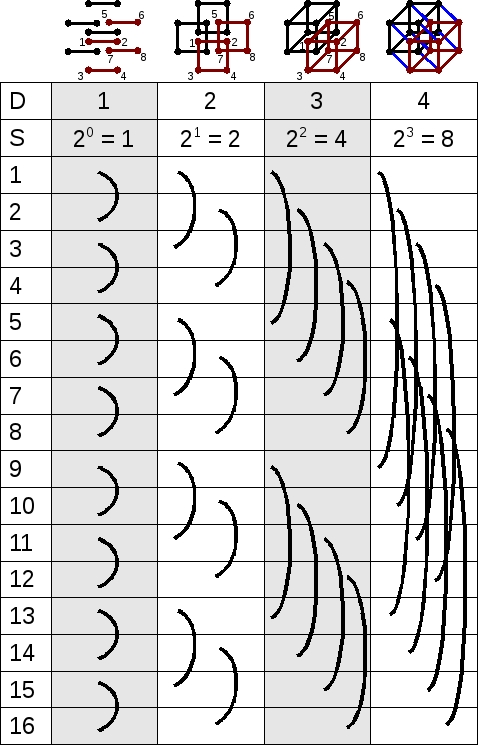
\includegraphics[width=0.5\linewidth]{images/theorie/hyper-build}
  \caption[Visuelle Darstellung des Algorithmus zur Erstellung eines Hypercube]{Darstellung des Algorithmus zur Erstellung eines Hypercube\index{Hypercube} der vierten Dimension. In jeder Dimension $D$ werden jeweils $S = 2^{D-1}$ Knoten nacheinander mit den $S$ n\"achsten Verbunden. Anschliessend werden $S$ Knoten \"ubersprungen und die noch ausstehenden wie vorhin verbunden. Codeblock \ref{alg:praxis-basis-hypercube-algemein} zeigt ein Code-Beispiel dieses Vorganges.}
  \label{fig:praxis-basis-hypercube}
\end{figure}

Zur Bildung eines Hypercube\index{Hypercube} muss zuerst die Dimension und die Anzahl Nodes bekannt sein. Die Dimension legt dabei fest, wie viele Verbindungen jede Node aufweist, also wie viele Schritte zur Berechnung notwendig sind. Bei einem Hypercube der dritten Dimension (ein W\"urfel) weist jede Node drei Verbindungen auf. Es sind also drei Durchg\"ange notwendig. Der Prozess f\"angt bei der ersten Node im ersten Durchgang an. Diese erste Node wird mit der nachfolgenden verbunden, also Node zwei. Da die zweite Node nun schon eine Verbindung aufweist, muss diese \"ubersprungen werden und mit der dritten weitergemacht werden. Diese wird anschliessend wiederum mit der nachfolgenden, also der vierten Node verbunden. Dieser Prozess wird so lange wiederholt bis alle Nodes eine Verbindung aufweisen.

Beim zweiten Durchlauf wird wieder mit der ersten Node angefangen, jedoch wird dieses mal nicht erneut eine Verbindung mit der zweiten Node hergestellt, sondern mit der Dritten. Die zweite Node besitzt noch keine zwei Verbindungen, also ist diese als n\"achste dran und wird mit der vierten Node verbunden. Node drei und vier weisen nun schon je zwei Verbindungen auf, es wird also mit der f\"unften Node weitergemacht und diese mit der Siebten verbunden. Nach dem zweiten Durchlauf weisen alle Nodes je zwei Verbindungen auf. Auf dem Papier w\"aren nun also zwei Quadrate zu sehen.

Diese beiden Quadrate m\"ussen im dritten Durchlauf nun zu einem W\"urfel zusammengesetzt werden, was wieder nach dem gleichen Prinzip geschieht. Begonnen wird wieder mit der ersten Node. Diese muss nun in die dritte Dimension verbunden werden, also mit der f\"unften Node. Die zweite Node muss eine Verbindung zur sechsten, die dritte eine zur siebten und die vierte eine zur achten Node aufbauen. Um die n\"achste Dimension zu verbinden, was dann die 4. Dimension w\"are, sind nicht mehr je vier Nodes zu verbinden und zu \"uberspringen, wie in der dritten, sondern je acht St\"uck.

Darauf aufbauend kann der Algorithmus in folgenden wenigen Aussagen zusammengefasst werden:
\begin{itemize}
 \item Im ersten Durchlauf wird jeder Knoten mit dem Nachfolgenden verbunden, wenn dieser nicht schon eine Verbindung aufweist. Es entstehen folgende Verkn\"upfungen: $1 \rightarrow 2$, $3 \rightarrow 4$, $5 \rightarrow 6$, $7 \rightarrow 8$, ...
 \item Im zweiten Durchlauf wird jeder Knoten mit dem \"ubern\"achsten verbunden, wenn dieser nicht schon eine Verbindung aufweist. Es entstehen folgende Verkn\"upfungen: $1 \rightarrow 3$, $2 \rightarrow 4$, $5 \rightarrow 7$, $6 \rightarrow 8$ ...
 \item Der dritte Durchlauf ist entsprechend, nur dass jeweils 3 Knoten ausgelassen werden. Die Verkn\"upfungen sind entsprechend: $1 \rightarrow 5$, $2 \rightarrow 6$, $3 \rightarrow 7$, $4 \rightarrow 8$ ...
 \item Im vierten Durchlauf werden dann nicht mehr 3 Knoten ausgelassen, sondern total sieben.
\end{itemize}
Pro Durchlauf m\"ussen also immer $2^{dimension-1}$ Nodes verbunden und anschliessend auch $2^{dimension-1}$ Nodes \"ubersprungen werden. Eine visuelle Darstellung des Prozesses ist in Abbildung \ref{fig:praxis-basis-hypercube} zu sehen. Aus der Grafik wird auch ersichtlich, dass die Spr\"unge pro Dimension jeweils um eine Zweierpotenz h\"oher sind.

\begin{figure}[h]
 \lstset{language=[ISO]C++}
 \begin{lstlisting}[label=alg:praxis-basis-hypercube-algemein,caption={[Algorithmus zur Erstellung eines Hypercubes]Algorithmus zur Erstellung eines Hypercubes\index{Hypercube} basierend auf einer Liste von Nodes. Die Pr\"ufung auf "`null"' bei der Verkn\"upfung behebt das Problem der leeren Knoten. Das Modulo mit der Anzahl existierender Knoten (Zeile 6) beim zu verbindenden Knoten gew\"ahrleistet, dass keine "`null"'-Node \"ubergeben wird und dass jede Node mehr als nur eine Verbindung aufweist.}]
for (dim = 0; dim < dimension; dim++) {
  dim_2 = Math.pow(2, dim);
  for (i = 0; i < num_nodes; i += (2*dim_2)) {
    for (j = 0; j < dim_2; j++)  {
      if (node_list[i+j] != null) {
        _n = (i + j + dim_2) % num_real_nodes;
        node_list[i + j].connectNode(list[_n]);
      }
    }
  }
}
 \end{lstlisting}
\end{figure}

Dieser Algorithmus kann in dieser Form einfach und schonend in ein Programm umgesetzt werden. Ein Beispiel zeigt Codeblock \ref{alg:praxis-basis-hypercube-algemein}, wobei bei dieser Implementierung zus\"atzlich noch leere Knoten ber\"ucksichtigt werden. Es wird davon ausgegangen, dass bei der Verbindung der Knoten durch die Funktion \texttt{connectNode(node)} geschaut wird, ob der \"ubergebene Knoten bereits eine Verbindung mit dem zu verbindenden Knoten aufweist oder nicht. Nur wenn noch keine Verbindung besteht, wird eine hergestellt (siehe Codeblock \ref{alg:praxis-basis-hypercube-connect}). W\"urde dies nicht gepr\"uft, k\"onnte ein Knoten mehrfach mit dem gleichen Knoten verbunden werden und es m\"usste mittels einem zus\"atzlichen Parameter definiert werden, ob der aktuelle Aufruf aus dem Algorithmus oder aus der Funktion kommt. Nur wenn der Aufruf direkt vom Algorithmus gemacht w\"urde, d\"urfte der \"ubergebene Knoten mit dem aktuellen verbunden werden (Zeile 12). Ansonsten w\"urden sich die Verbindungsfunktionen auf den zwei Knoten endlos gegenseitig aufrufen.

\begin{figure}[h]
 \lstset{language=[ISO]C++}
 \begin{lstlisting}[label=alg:praxis-basis-hypercube-connect,caption={[Verbinden von zwei Hypercube-Nodes]Die Funktion, welche zwei Knoten verbindet, pr\"uft zuerst ob der Knoten nicht schon in der Liste vorhanden ist. Wenn nicht, wird der Knoten eingef\"ugt und die gleiche Funktion auf dem zu verbindenden Knoten aufgerufen. Ohne diese Pr\"ufung w\"urde hier eine endlose Aufruf-Aktion stattfinden.}]
if (node == null) return;
if (node == this) return;
bool connected = false;
foreach (HyperNode c_node in node_list) {
  if (c_node == node) {
    connected = true;
    break;
  }
}
if (!connected) {
  node_list.append(node);
  node.connectNode(this);
}
 \end{lstlisting}
\end{figure}

\subsection{Versenden von Alert-Nachrichten} \label{sec:praxis-basis-sendalert}
Das Problem der mehrfachen Meldungs-Zustellung wurde bereits in Kapitel \ref{sec:theorie-alert} diskutiert und dazu eine akzeptable L\"osung gefunden. Das System schaut in einem ersten Schritt in der Datenbank nach, wann dieser Alert (basierend auf Host und Modul) zuletzt gesendet worden ist. Anhand des Zeitstempels sowie des Pr\"ufintervals wird dann entscheiden, ob die aktuelle Meldung notwendig ist oder nicht.

Die Benachrichtigung, welches Modul bei welchem System fehlgeschlagen ist, wird durch den \texttt{MainListener} empfangen und durch das \texttt{MainSystem} in die Datenbank eingetragen. Die Alert-Funktion \texttt{sendAlert} liest diese Daten aus und entscheidet, ob eine Meldung versendet werden soll. Soll ein Alert versendet werden, wird dies zuerst den anderen \"Uberwachungssystemen mitgeteilt und anschliessend die Alert-Meldung versendet. In Abbildung \ref{fig:alert-sample} wird zuerst die Meldung versendet und anschliessend die anderen Systeme dar\"uber informiert. Dies kann jedoch dazu f\"uhren, dass eine Meldung mehrfach versendet wird, denn w\"ahrend das eine System eine Nachricht sendet, k\"onnen andere den Ausfall ebenfalls bemerken und eine Meldung versenden.

Grunds\"atzlich w\"urde eine Meldung unter Umst\"anden alle paar Sekunden versendet werden, denn bei der ausgearbeiteten L\"osung wird nur basierend auf dem Pr\"ufungsintervall eine Pause definiert. Um diesem Problem Herr zu werden, wird versucht heraus zu finden, wie lange das System bereits nicht mehr auf den Dienst reagiert. Basierend auf dieser Anzahl Sekunden kann anschliessend ein Alert-Plan geladen werden.

Ein Alert-Plan, definiert durch die \texttt{AlertConfig}-Klasse, beschreibt, wie mit einem Ausfall bei einem Modul und System sowie der entsprechenden Downtime umgegangen werden soll. Die Konfiguration beinhaltet den Namen des \"Uberwachungsmodules, die Sekundenwerte "`von"' und "`bis"' zur Definierung der Downtime, ein Timeout in Sekunden sowie eine Liste von Empf\"angern. Basierend auf dem Timeout und der letzten Alert-Meldung kann somit gesagt werden, ob oder wann eine Meldung versendet werden soll.

In der f\"ur die Bachelor-Thesis ausgearbeiteten Technologie-Demonstration wird der Alert-Plan eine statische Liste von Werten sein. In einer zuk\"unftigen Version wird diese global pro Dienst definiert und auf Systemebene noch verfeinert werden k\"onnen. Es kann zuk\"unftig somit bestimmt werden, welcher Dienst \"uber welches Alert-Modul bei welchen Personen eine Benachrichtigung hinterlassen soll.


%%%%%%%%%%%%%%%%%%%%%%%%%%%%%%%%%%%%%%%%%%%%%%%%%%%%%%%%%%%%%%%%%%%%%%%%%%%%%%%%%%%%%%%%%%%%%%%%%%%%%%%%%%%%%%%%%%%%%%%%%%%%%%%%%%%%%%%%%
\section{Einfache Installation und Konfiguration} \label{sec:praxis-install}
In einer finalen Version sollte das Produkt nicht nur als bin\"are Version, sondern auch als Quellcode verf\"ugbar sein. Die Voraussetzung f\"ur die Compilierung ist nicht nur ein aktueller Vala- sondern auch ein C-Compiler. Zus\"atzlich m\"ussen noch verschiedene Libraries wie die GLib, GEE und GIO vorhanden sein, sowie Datenbank-Bibliotheken f\"ur die verschiedenen Module. Sind alle Voraussetzungen gegeben, kann der Quellcode durch GNU-Make kompiliert und anschliessend verwendet werden.

Ist das Produkt in einer bin\"aren Form vorhanden, muss dieses nur in einen Ordner kopiert und kann dort direkt gestartet werden. Die Grundkonfiguration, also welche Datenbank-Engine genutzt werden soll, kann \"uber einen Startparameter definiert werden. Andere Einstellungen m\"ussen nicht get\"atigt werden. Damit das Programm beim Systemstart automatisch gestartet wird, muss nur noch ein entsprechendes Kommando in den Startprozess eingef\"ugt werden. Dieser ist nicht nur plattformabh\"angig sondern auch unter Linux/BSD/Unix unterschiedlich von Distribution zu Distribution.

Um ein System in die \"Uberwachung mit auf zu nehmen, muss dieses \"uber eine Weboberfl\"ache oder ein anderes Remote-API-Modul konfiguriert werden. Diese Grundkonfiguration kann dabei auf zwei unterschiedliche Arten erfolgen:

\begin{description}
 \item[\"Uber eine direkte Verbindung] kann dem neuen System mitgeteilt werden, welche IP-Adresse es hat und in welchem Netzwerk es ist. Soll das System in ein bestehendes \"Uberwachungsnetzwerk eingebunden werden, muss dem neuen System nur ein anderes im gleichen Netzwerk vorhandenes System angegeben werden. Ist in dem neuen Netzwerk kein anderes System vorhanden, m\"ussen eventuelle weitere Parameter angegeben werden, um zum Beispiel eine OpenVPN-Verbindung\index{VPN!OpenVPN} aufbauen zu k\"onnen.

 \item[\"Uber ein anderes System] kann das neue System ebenfalls eingebunden werden. Auf einem System kann \"uber ein Remote-API-Modul ein neues System durch die Angabe von IP-Adresse und Netzwerk eingebunden werden. Diese Methode funktioniert jedoch nicht, wenn das neue System das einzige in einem neuen Netzwerk ist, denn dieses besitzt noch keine OpenVPN-Daten und Verbindungen.
\end{description}

Ist das neue System erst einmal im Netzwerk registriert, kann die Konfiguration an diesem vorgenommen werden. Durch einfache Prozessabl\"aufe k\"onnen verschiedene Dienste konfiguriert werden. Sind alle Parameter und Dienste eines Systems konfiguriert, kann durch eine Synchronisation das entsprechende System aktualisiert werden. Eine solche Synchronisation sollte jedoch erst nach Beendigung der Konfiguration durchgef\"uhrt werden, denn durch eine Einbindung eines neuen Systems oder Dienstes, wird eine komplette Neubildung des Hypercubes f\"allig.

Die grundlegenden Konfigurationen wie die globalen und lokale Datenbanken, VPN-Daten etc. werden ebenfalls mittels den Remote-API-Modulen konfiguriert. Bei der Synchronisation von diesen wird aber in den meisten F\"allen kein Rebuild des Hypercubes notwendig. Eine Reinitialisierung des Management-Netzwerkes oder des Systems ist m\"oglich.

\subsection{M\"ogliche Funktionen einer Konfigurationsoberfl\"ache} \label{sec:praxis-install-conf}
Eine Konfigurationsoberfl\"ache sollte wenn m\"oglich die nachfolgenden Funktionen und Bereiche aufweisen:

\begin{description}
 \item[Grundkonfiguration:] Die Grundkonfiguration beinhaltet alle Basis-Parameter und Definitionen. Dies sind zum Beispiel globale Parameter der einzelnen \"Uberwachungsmodule wie ein Timeout bei einem ECHO-Request, welche Datenbank als Standard verwendet wird, ob und welche Datenbank als globaler Datenbank-Mirror/Backbone verwendet wird, etc.

 \item[Netzwerke:] Die Netzwerk-Konfiguration definiert in erster Linie das Netzwerk anhand einer IP-Adresse und einer Subnet-Maske. Zus\"atzlich werden noch Parameter f\"ur die Herstellung eines OpenVPN-Management-Netzwerkes\index{VPN!OpenVPN} sowie eine Gateway-Adresse definiert, \"uber welche die anderen Netzwerke kommunizieren k\"onnen.

 \item[Network-Discovery:] Das Network- oder auch Host-Discovery dient in erster Linie dazu, neue Systeme in einem Netzwerk zu finden und diese zu untersuchen. Die so gefundenen Systeme k\"onnen anschliessend \"uber die \textbf{Host-Konfiguration} bearbeitet werden.

 \item[Host-Konfiguration:] Dieser Bereich listet alle Systeme und deren \"uberwachten Dienste auf. Auf den einzelnen Systemen k\"onnen neue Dienste hinzugef\"ugt, entfernt oder bearbeitet werden. Die globale System-Konfiguration wie IP-Adresse, Netzwerk, usw. sollte ebenfalls dar\"uber konfigurierbar sein.
\end{description}

\subsection{Installation der TechDemo} \label{sec:praxis-install-demo}
Die Technologie-Demonstration soll die Machbarkeit aufzeigen und nicht ein voll funktionst\"uchtiges Produkt darstellen. Zur Pr\"ufung der Funktionalit\"at werden relativ viele Informationen auf der Konsole ausgegeben.

Die Technologie-Demonstration erfordert aktuell mehr Konfigurationsaufwand als die geplante finale Version. Dazu notwendig ist ein Sqlite3-Datenbank-Programm wie SQLiteMan (\url{http://www.sqliteman.com/}) um verschiedene Systeme in die \"Uberwachung auf zu nehmen. Die TechDemo wird in zwei Bin\"ar-Versionen angeboten (32-Bit POSIX, 64-Bit POSIX) sowie auch als Vala-Sourcecode. Eine Windows-Version ist aktuell nicht vorhanden.

Die bin\"aren Versionen k\"onnen aus einem beliebigen Verzeichnis gestartet werden. Als Startparameter werden die IP-Adresse als Dot-String sowie die Subnet-Maske als numerischer Wert ben\"otigt: \texttt{./modules 1.2.3.4 24}

Vor dem ersten Start sollte die Datei "`dummy\_alert\_config.txt"' im data-Ordner bearbeitet werden. Diese beinhaltet momentan die Konfiguration f\"ur das EMail-Alert-Modul. Die Parameter sollten selbstbeschreibend sein, eine Auflistung und Beschreibung ist aber im Anhang in Tabelle \ref{tbl:praxis-install-dummyalertconf} zu sehen. Anschliessend muss die Sqlite-Datenbank "`config.sqlite"', ebenfalls im data-Verzeichnis, bearbeitet werden. In der Tabelle "`networks"' muss in einem ersten Schritt das bestehende Netzwerk angepasst und allenfalls zus\"atzliche eingetragen werden. In der Tabelle "`hosts"' m\"ussen alle anderen \"Uberwachungssysteme eingetragen werden. Die Tabelle "`modules"' schlussendlich beinhaltet alle Systeme, welche \"uberwacht werden sollen. Jede Zeile in der "`modules"' Tabelle steht f\"ur einen Parameter. Es werden somit zwei Zeilen ben\"otigt, wenn ein System mittels \texttt{icmp} alle 5 Sekunden (timeout) und je 2 Echo-Requests (num) \"uberwacht werden soll.

Sind alle Konfigurationen gemacht, kann das System, wie oben angegeben, gestartet werden. Kommandos k\"onnen anschliessend mittels "`netcat"' (siehe Kapitel \ref{sec:praxis-basis-kernel-listener}) dem System \"ubergeben werden. Mit der Erstellung von Test-Hosts sollte vorsichtig umgegangen werden. Da Sqlite nicht gerade die schnellste Datenbank ist, kann zum Beispiel die Erstellung eines /16-er Netzwerkes mit mehreren tausend Systemen einige Minuten in Anspruch nehmen.

Alternativ kann auch mittels einem aktuellen Firefox oder einem auf KHTML/WebKit basierenden Browser wie Chrome oder Safari eine Konfiguration \"uber das JSON-RPC-Modul vorgenommen oder ge\"andert werden. Hierf\"ur muss die die Datei "`json-rpc.html"' aus dem "`demo"'-Verzeichnis ge\"offnet werden. Der erste Dialog dient zur Angabe eines laufenden Systems, wobei als Standard-Port f\"ur JSON-RPC momentan der Port 2784 (www-dev) verwendet wird. Die Oberfl\"ache dieser Demo-Weboberfl\"ache sollte weitgehenst selbsterkl\"arend sein: Im linken Bereich werden alle Netzwerke und durch einen Klick auf ein solches auch die Systeme angezeigt. Durch einen klick auf ein System werden mittig die System-Konfigurationen dargestellt und rechts ein Kommunikations-Log. Oberhalb wird eine Menubar/Symbolleiste angezeigt, \"uber welche verschiedene Aktionen ausgef\"uhrt werden k\"onnen. Wichtig bei der Ben\"utzung zu wissen ist, dass der Server teilweise keine Verbindungen annimmt, was zu Fehlern f\"uhren kann. Wird ein solcher Fehler gezeigt muss unter umst\"anden die Seite neu geladen werden, da die Browser erst anschliessend wieder in der Lage sind eine Verbindung herzustellen.

Ein Problem bei der aktuellen Version stellt ein Speicherfehler in der SQLite3-Bibliothek dar. Bei der Verwendung von \texttt{Sqlite3.Statement} beim auslesen von Daten, werden Speicherbereiche nicht mehr korrekt fereigegeben. Dies hat zur Folge dass durch den Betrieb der \"Uberwachungs-Software aktuell immer mehr Speicher (heap) verbraucht wird und nicht wiederverwendet werden kann. Durch die Verwendung von Sqlite3 als externe Bibliothek, kann es durchaus sein, dass dieser Fehler nicht auf jeder Installation vorhanden ist.

\section{Verschiedene Szenarien} \label{sec:praxis-businesscases}
Zur Veranschaulichung der Technologie-Demonstration werden in diesem Kapitel einige Szenarien nachgespielt sowie die Reaktion des Systems darauf gezeigt.

\subsection{Rebuild eines Hypercubes}
Damit der Prozess der Bildung eines Hypercube besser gezeigt werden kann, wird eine Datenbank mit 20 Pseudo-Systemen aus dem Subnet "`192.168.22.0/24"' verwendet. Diese Dummy-Hosts werden durch den Befehl \texttt{echo '1   1   a8812636a6ad0b84ab8f6943728551a4""testdata: 192.""168.""22.0 24 20' \textbar nc -q1 -u 192.""168.""22.""27 1611} angelegt und durch \texttt{echo '1   1   a8812636a6ad0b84ab8f6943728551a4""rebuild:' \textbar nc -q1 -u 192.""168.""22.""27 1611} neu gebildet.

\begin{figure}[H]
  \centering
  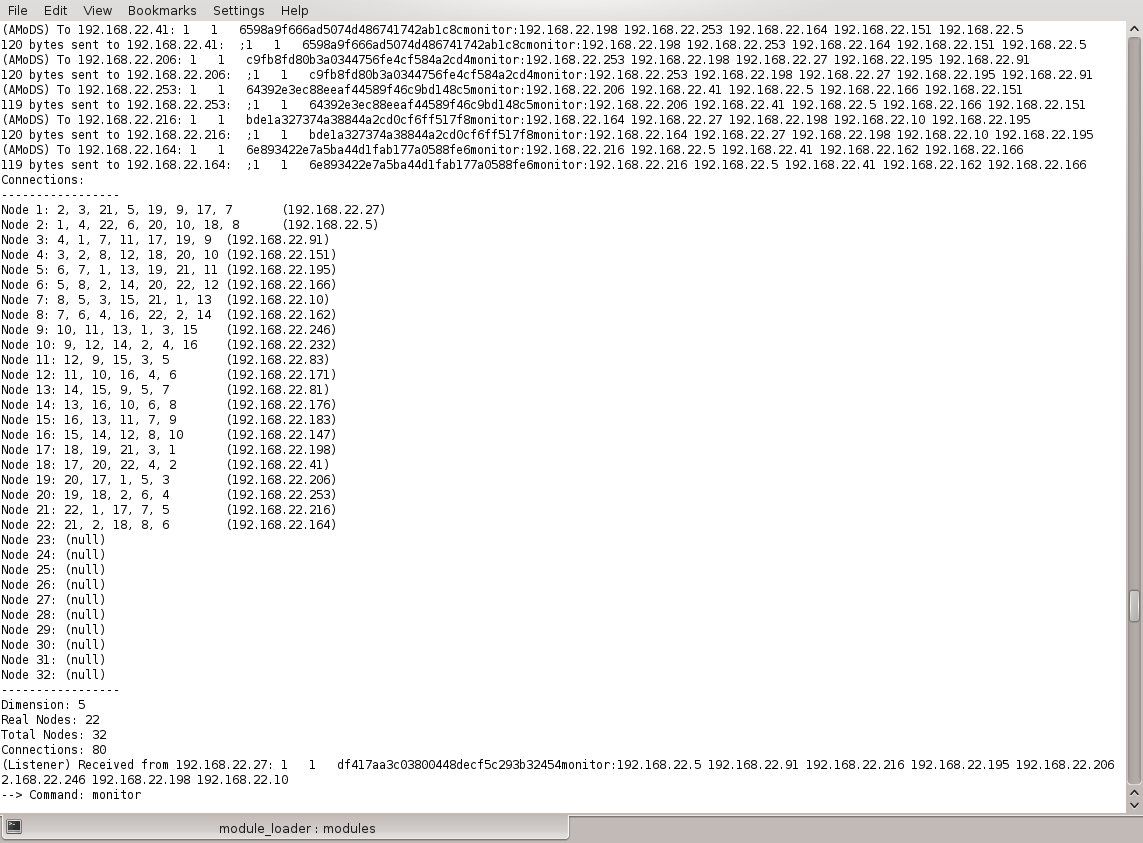
\includegraphics[width=0.9\linewidth]{images/theorie/amods_rebuild}
  \caption[Erstellen von DummyHosts und Rebuild des Hypercubes]{Im oberen Bereich sind Nachrichten sichtbar, welche die anderen Systeme dar\"uber informieren, welche anderen Systeme sie \"uberwachen m\"ussen. Der mittlere Bereich zeigt den Hypercube, respektive alle gemachten Verbindungen zwischen den Systemen. Unten angef\"ugt werden noch die Hypercube-Daten gezeigt. Die letzten Zeilen zeigen die eingegangene Nachricht, welche dem aktuellen System mitteilt, welche anderen Systeme es \"uberwachen muss.}
  \label{fig:nat-source}
\end{figure}

\textbf{Achtung:} Wenn Systeme manuell in die Datenbank eingetragen worden sind, die nicht im gleichen Netzwerk wie der aktuelle Server sind, werden diese aus der \"Uberwachung entfernt. Es wird nicht das System an sich entfernt, sondern nur die Eintr\"age in der "`modules"'-Tabelle, welche alle \"uberwachten Systeme beinhaltet.

\subsection{Ausfall eines Systems}
F\"allt ein System aus und wird ein Alert versendet, wird dies allen anderen Systemen mitgeteilt. Zus\"atzlich ist in diesem Szenario noch ein Konfigurationsfehler, welcher das senden einer Alert-Meldung nicht zul\"asst. Dieser Fall wird in der TechDemo jedoch nicht abgefangen, denn es wird grunds\"atzlich davon ausgegangen, dass ein Alert versendet werden kann.

\begin{figure}[H]
  \centering
  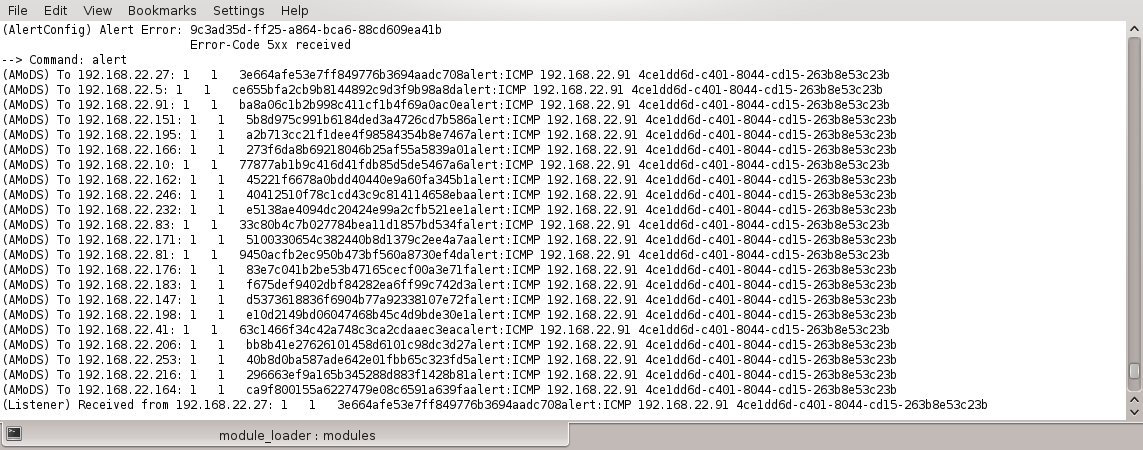
\includegraphics[width=0.9\linewidth]{images/theorie/amods_ausfall}
  \caption[Ausfall eines Systems]{Die ersten Zeilen zeigen auf, dass der Alert nicht versendet werden konnte. Der EMail-Server hat einen 5xx-Code als Antwort gesendet. Die anschliessenden Zeilen zeigen die Nachrichten an alle weiteren Systeme, welche informiert werden, dass der Alert mit der ID \textbf{4ce1dd6d-c4...} f\"ur das System \textbf{192.168.22.91} und Plugin \textbf{ICMP} versendet worden ist. Die letzte Zeile zeigt auf, dass das laufende System die oben gesendete Nachricht auch empf\"angt und weiterverarbeitet.}
  \label{fig:nat-source}
\end{figure}

Wird ein Systemfehler entdeckt, ein Alert wurde jedoch schon gesendet, wird so lange gewartet, bis wieder ein Alert versendet werden darf.

\begin{figure}[H]
  \centering
  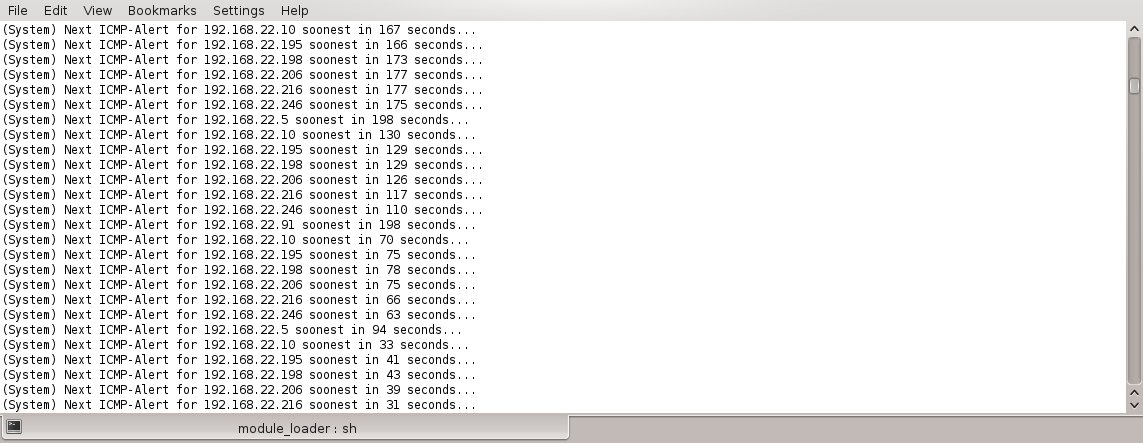
\includegraphics[width=0.9\linewidth]{images/theorie/amods_waiting}
  \caption[Warten beim Ausfall eines Systems]{Wird das Senden eines Alerts beim auffinden eines Problems durch eine Semaphore geblockt, wird dies aktuell durch die Wartezeit angezeigt.}
  \label{fig:nat-source}
\end{figure}


\subsection{\"Uberwachung eines EMail-Servers}
Wird bei der SMTP-Modul-Konfiguration ein Fehler gemacht, wird dies aktuell nicht erkannt, sondern es wird angenommen, dass etwas mit dem System nicht in Ordnung ist.

\begin{figure}[H]
  \centering
  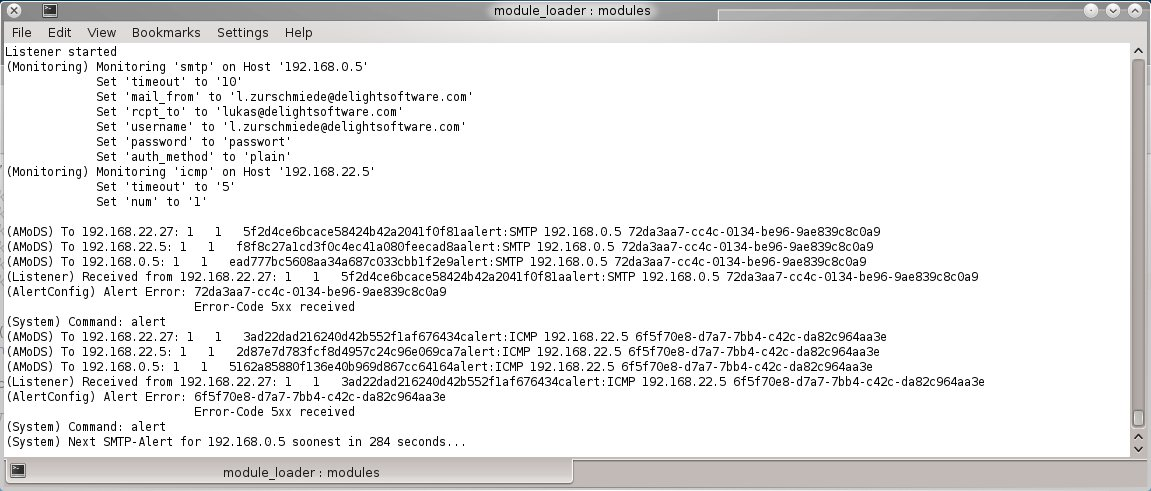
\includegraphics[width=0.9\linewidth]{images/theorie/amods_email_error}
  \caption[Fehler beim \"uberwachen eines EMail-Servers]{Auf den ersten Zeilen wird gezeigt, mit welchen Parametern das SMTP-Modul geladen wird. Das fehlerhaft Passwort verursacht eine Alert-Meldung, welche anschliessend auf die umliegenden Systeme verteilt wird.}
  \label{fig:nat-source}
\end{figure}



